\documentclass[12pt]{article}
\thispagestyle{empty}
\usepackage{amsmath}
\usepackage[margin=1in]{geometry}
\usepackage{amsfonts}
\usepackage{hyperref}
\usepackage{graphicx}
\usepackage{siunitx}
\usepackage{cancel}
\usepackage{xfrac}
\usepackage{listings}
\usepackage{longdivision}

\begin{document}
	
	\begin{center}
		\par\noindent \large \textbf{Hexadecimals (part 3)}  [ Andy Chong Sam ]
	\end{center}
	\begin{minipage}[t]{.5\linewidth}
		\par\noindent\textbf{(I)} In this article we'll discuss how hexadecimals are used in Cascading Style Sheets (CSS) to describe color. For reference, the hexadecimal chart is provided below.  
		\begin{center}
			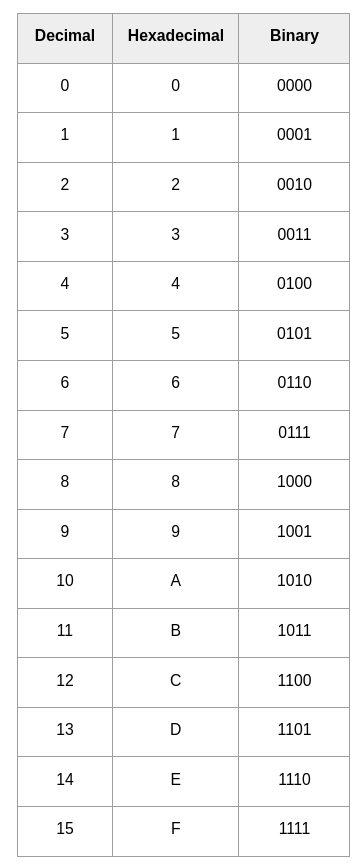
\includegraphics[width=4.0cm]{hex-chart.png}
		\end{center}
		\par\noindent The RGB model is an additive color model in which red, green, and blue are combined in various intensities to produce all other colors. The intensity of each color is described as an unsigned integer ranging from 0 to 255 inclusive. We will describe the value for each color as a triplet (r, g, b).
		\newline
		\par\noindent Some color definitions are shown here:
\begin{center}
	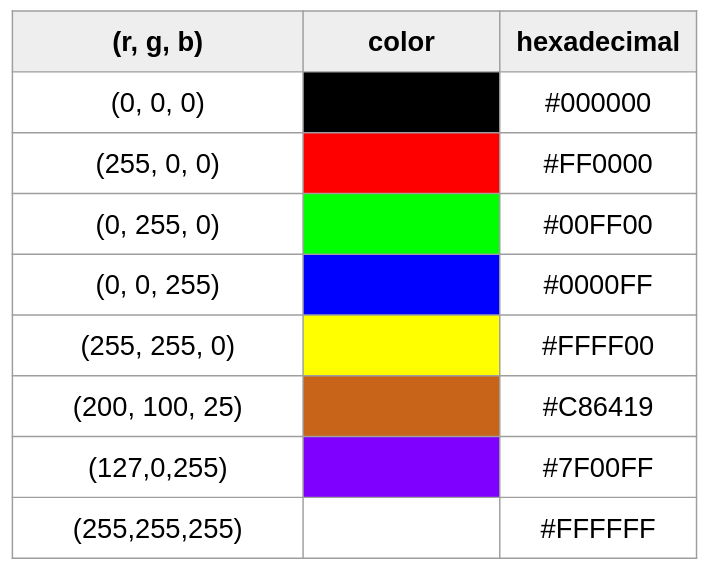
\includegraphics[width=5.5cm]{rgb.png}
\end{center}
	\end{minipage}	
	\hspace{0.45cm}
	\begin{minipage}[t]{.5\linewidth} 
		
		\par\noindent\textbf{(II)} When creating CSS code, one can optionally use hexadecimal values instead of RGB triplet combinations. Note that in CSS code, hexadecimals are prefixed with the \# symbol, a convention we will follow here. Let's calculate the hexadecimal value for 255:
		\begin{flalign*}
			\intlongdivision{255}{16}\;\;\intlongdivision{15}{16}
		\end{flalign*}
		\par\noindent The reverse remainder sequence is 15 and 15, giving us a hexadecimal of FF. Recall that the hexadecimal symbol for 15 is F. Since the decimal range is 0 to 255 inclusive, then the hexadecimal range is 00 to FF. We can therefore say for example that the rgb triplet (255, 255, 255) is the same as \#FFFFFF.
		\newline
		\par\noindent\textbf{(III)} Let's confirm the hexadecimal value for (12, 0, 255). We already know that 255 is FF, and 0 is 00, so what's left is to figure out 127:
		\begin{flalign*}
			\intlongdivision{127}{16}\;\;\intlongdivision{7}{16}
		\end{flalign*}
		\par\noindent If we reverse the remainder sequence of 15 and 7, we get 7F. So the hexadecimal representation of (127,0,255) is \#7F00FF.
	
	\end{minipage}
	
\end{document}